% ---------
% --------
%!TEX TS-program = pdflatex
%!TEX encoding = UTF-8 Unicode
%!TEX spellcheck = English (Aspell)

\documentclass[11pt]{article}
\usepackage{jeffe,handout,graphicx}
\usepackage{fourier-orns}
\usepackage{mathtools}
\usepackage[normalem]{ulem} % either use this (simple) or
\usepackage{tikz}

\def\Cdot{\mathbin{\text{\normalfont \textbullet}}}
\def\Sym#1{\texttt{\color{BrickRed}#1}}
\def\BlueSym#1{\textbf{\texttt{\color{RoyalBlue}#1}}}
\allowdisplaybreaks

\begin{document}

\begin{center}
\Large\textbf{CSCI 432/532, Spring 2026}%
\\
\LARGE\textbf{Homework 2}%
\\[0.5ex]
\large Due Monday, February 2 at 9am
\end{center}

\bigskip
\hrule
\bigskip

\subsection*{Submission Requirements}
\begin{itemize}
    \item Type or clearly hand-write your solutions into a PDF format so that they are legible and professional. Submit your PDF on Gradescope. 
    \item Do not submit your first draft. Type or clearly re-write your solutions for your final submission. If your submission is not legible, we will ask you to resubmit.
    \item Use Gradescope to assign problems to the correct page(s) in your solution. If you do not do this correctly, we will ask you to resubmit.
\end{itemize}

\subsection*{Collaboration and Resources}

The \emph{best} resources for completing the homework are (in no particular order):
\begin{itemize}
	\item Your own notes from lectures and problem sessions, and/or lecture recordings.
	\item The lecture notes linked from the course website for the lecture day.
	\item The questions channel on Discord.
	\item Office hours.
	\item Discussions with classmates.
\end{itemize}
You may also access almost any resource in preparing your solution to the
homework. The exception is that you may not seek answers to the problems on the
homework directly, such as by pasting them into a GenAI tool, searching for
solutions on a search engine, looking for them on Chegg or similar websites, or
asking another person for the solution.

 However, you \EMPH{must}
\begin{itemize}
    \item Write your solutions in your own words---this means that you should never be \emph{copying}
    anything of substance from any source, and
    \item credit every resource you use, including GenAI tools, by providing links or full chat transcripts.
    If you use the provided LaTeX template, you can use the \texttt{Sources}
    environment for this. Ask if you need help!
\end{itemize}


\begin{boxquote}{0.9}
Remember, if you choose to use GenAI tools, not only must you provide a full
transcript of your conversation (or a link to one), you must also use the
following prompt (or some variation of it), and provide a full transcript of
the conversation.
\end{boxquote}  

Prompt:
\begin{boxquote}{0.9}
You are acting as a teaching assistant for an advanced undergraduate/graduate
algorithms and computer science theory course.

Your role is not to provide full solutions or final answers.

Instead, you should act like we are having a conversation. Ask me a single
question and let me respond. Avoid asking me many questions at once or giving
me a lot of information at one time. Guide me using hints, leading questions,
partial insights, and sanity checks.  Help me debug my own proofs, algorithms,
or reductions. Do not give a complete solution or full proofs. Be patient with
me. Don't give me details so that I can move on to the next part of a problem.
Make sure that I understood before moving on.

The course uses Jeff Erickson's Models of Computation lecture notes, so you should
guide me to answer problems using the definitions, notation, and style from those notes.

Assume I am a serious student trying to learn, not to shortcut the assignment.
I am attaching the assignment, so you should refuse to provide a complete solution
to the problems listed. Of course, you can walk me through the "Solved
Problems" listed at the end if I ask.
\end{boxquote}  



\newpage
%----------------------------------------------------------------------

\headers{CSCI 432/532}{Homework 2 (due February 2)}{Spring 2026}

\begin{enumerate}
%\parindent 1.5em \itemsep 4ex plus 0.5fil

%----------------------------------------------------------------------

\item
For each of the following languages over the alphabet $\Sigma = \{\Sym0, \Sym1 \}$, give an equivalent regular expression, and briefly explain why your regular expression is correct. Note that there are infinitely many correct answers for each language.

\begin{enumerate}[(a)]
    \item (3 points) All strings that begin with the prefix \Sym{001}, end with the suffix \Sym{100}, and contain an odd number of \Sym1's.
    \item (3 points) All strings that contain both \Sym{0011} and \Sym{1100} as substrings. 
    \item (4 points) All strings that contain the substring \Sym{01} an odd number of times.
\end{enumerate}

\begin{Rubric}{Regular expression rubric}

10 points =
\begin{itemize}
    \item[+ 2] for a syntactically correct regular expression.
    \item[+ 4] for a brief English explanation of your regular expression. This is how you
argue that your regular expression is correct.
\begin{itemize}
    \item For longer expressions, you should explain each of the major components of your expression,
and separately explain how those components fit together.
\item We do not want a transcription; don’t just translate the regular-expression notation into English.
\end{itemize}
    \begin{itemize}
        \item Yes, you need to write it down. Yes, even if it’s ``obvious''. Remember that the goal of the homework is to communicate with people who aren't as clever as you.
    \end{itemize}
    \item[+ 4] for correctness.
    \begin{itemize}
        \item $-4$ for incorrectly answering $\emptyset$ or $\Sigma^*$.
        \item $-1$ for a single mistake: one typo, excluding exactly one string in the target language, or including exactly one string not in the target language. (The incorrectly handled string is almost always the empty string $\e$.)
        \item $-2$ for incorrectly including/excluding more than one but a finite number of strings.
        \item $-4$ for incorrectly including/excluding an infinite number of strings.
    \end{itemize}
\item Regular expressions that are more complex than necessary may be penalized. Regular expressions that
are significantly too complex may get no credit at all. On the other hand, minimal regular expressions
are not required for full credit.
\end{itemize}
\end{Rubric}

\item For each of the following languages over the alphabet $\Sigma = \{\Sym0, \Sym1\}$, describe a DFA that
accepts the language, and briefly describe the purpose of each state. You can describe
your DFA using a drawing or using formal mathematical notation.

\begin{enumerate}[(a)]
    \item All strings in $\Sym1^*\Sym0\Sym1^*$.
    \item All strings containing the substring \Sym{01010010}.
    \item  All strings that represent a multiple of 5 in base 3. For example, this language contains
the string \Sym{10100}, because $\Sym{10100}_3 = 90_{10}$ is a multiple of 5. (In general, numbers in base 3 could contain the symbol \Sym2, but those are excluded from this language.)
\emph{Hint: take a look at 3.1 in the textbook: \url{https://umaal.org/teaching/cscix32-spring-2026/lectures/03-automata.pdf}.}
\end{enumerate}
\begin{Rubric}{NFA/DFA rubric}
10 points =
\begin{itemize}
    \item[+ 2] for an unambiguous description of a DFA or NFA, including the states set $Q$, the start state $s$,
the accepting states $A$, and the transition function $\delta$.
  
\begin{itemize}
\item Drawings:
\begin{itemize}
\item Use an arrow from nowhere to indicate the start state s.
\item Use doubled circles to indicate accepting states A.
\item If $A = \emptyset$, say so explicitly.
\item If your drawing omits a junk/trash/reject/hell state, say so explicitly.
\item Draw neatly! If we can’t read your solution, we can’t give you credit for it.
\end{itemize}
\item Text descriptions: You can describe the transition function either using a 2d array, using mathematical notation, or using an algorithm.
\begin{itemize}
\item You must explicitly specify $\delta(q, a)$ for every state $q$ and every symbol $a$.
\item If you are describing an NFA with $\e$-transitions, you must explicitly specify $\delta(q, \e)$ for every
state q.
\item If you are describing a DFA, then every value $\delta(q, a)$ must be a single state.
\item If you are describing an NFA, then every value $\delta(q, a)$ must be a set of states.
\item In addition, if you are describing an NFA with $\e$-transitions, then every value $\delta(q, \e)$ must
be a set of states.
\end{itemize}
\item Product constructions: You must give a complete description of each of the DFAs you are combining (as either drawings, text, or recursive products), together with the accepting states of the
product DFA. In particular, we will not assume that product constructions compute intersections
by default.
\end{itemize}
\item[+ 4] for briefly explaining the purpose of each state in English. This is how you
argue that your DFA or NFA is correct.
\begin{itemize}
\item In particular, each state must have a mnemonic name.
\item For product constructions, explaining the states in the factor DFAs is both necessary and sufficient.
\item Yes, we mean it. A perfectly correct drawing of a perfectly correct DFA with no state explanation
is worth at most 6 points.
\end{itemize}
\item[+ 4] for correctness. 
\begin{itemize}
\item $-1$ for a single mistake: a single misdirected transition, a single missing or extra accepting state,
rejecting exactly one string that should be accepted, or accepting exactly one string that should
be accepted. (The incorrectly accepted/rejected string is almost always the empty string $\e$.)
\item $-4$ for incorrectly accepting every string, or incorrectly rejecting every string.
\item $-2$ for incorrectly accepting/rejecting more than one but a finite number of strings.
\item $-4$ for incorrectly accepting/rejecting an infinite number of strings.
\end{itemize}
\end{itemize}
\end{Rubric}

\end{enumerate}

% ===========================================================================
\newpage

\def\ForceSym#1{\setbox0\hbox{A}\hbox to \wd0{\hss #1\hss}}
\def\Blank{\ForceSym{$\diamond$}}
\def\Enter{\ForceSym{\rotatebox[origin=c]{180}{$\Rsh$}}}	% Better
\def\Var#1{\ensuremath{\seq{\textsf{#1}}}}

\subsection*{Solved problems}

\def\CPP{{C\nolinebreak[4]\hspace{-.05em}\raisebox{.33ex}{\tiny\bf ++}}}

\begin{enumerate}\setcounter{enumi}{3}
\item
\EMPH{C comments} are the set of strings over alphabet $\Sigma = \Set{\Sym{*},
\Sym{/}, \Sym{A}, \Sym{\Blank}, \Sym{\Enter} }$ that form a proper comment in
the C program language and its descendants, like \CPP\ and Java.
Here~$\Sym{\Enter}$ represents the newline character, $\Sym{\Blank}$ represents
any other whitespace character (like the space and tab characters), and \Sym{A}
represents any non-whitespace character other than~$\Sym{*}$~or~$\Sym{/}$.%
% ======
\footnote{The actual C commenting syntax is considerably more complex than described here, because of character and string literals.
%
\begin{itemize}\cramped
\item
The opening \Sym{/*} or \Sym{//} of a comment must not be inside a string literal ($\Sym{"}\cdots\Sym{\textquotedbl}$) or a (multi-)character literal ($\Sym{\textquotesingle}\cdots\Sym{\textquotesingle}$).
\item
The opening double-quote of a string literal must not be inside a character literal (\Sym{\textquotesingle"\textquotesingle}) or a comment.
\item
The closing double-quote of a string literal must not be escaped (\Sym{\textbackslash"})
\item
The opening single-quote of a character literal must not be inside a string literal ($\Sym{"}\cdots\Sym{\textquotesingle}\cdots\Sym{\textquotedbl}$) or a comment.
\item
The closing single-quote of a character literal must not be escaped (\Sym{\textbackslash'})
\item
A backslash escapes the next symbol if and only if it is not itself escaped (\Sym{\textbackslash\textbackslash}) or inside a comment.
\end{itemize}
%
For example, the string $\Sym{"/*\textbackslash\textbackslash\textbackslash"*/"/*"/*\textbackslash"/*"*/}$ is a valid string literal (representing the 5-character string \Sym{/*\textbackslash"\textbackslash*/}, which is itself a valid block comment!\@) followed immediately by a valid block comment.  \EMPH{For this homework question, just pretend that the characters \Sym{\textquotesingle}, \Sym{"}, and \Sym{\textbackslash} don't exist.}

Commenting in \CPP\ is even more complicated, thanks to the addition of \emph{raw} string literals.  Don't ask.

Some C and \CPP\ compilers do support nested block comments, in violation of the language specification. A few other languages, like OCaml, explicitly allow nesting block comments.
}
% ======
%
There are two types of C comments:
\begin{itemize}
\item Line comments:  Strings of the form $\Sym{//} \cdots \Sym{\Enter}$
\item Block comments:  Strings of the form $\Sym{/*} \cdots \Sym{*/}$
\end{itemize}
%
Following the C99 standard, we explicitly disallow \EMPH{nesting} comments of the same type.  A~line comment starts with $\Sym{//}$ and ends at the first $\Sym{\Enter}$ after the opening $\Sym{//}$.  A block comment starts with $\Sym{/*}$ and ends at the the first $\Sym{*/}$ completely after the opening $\Sym{/*}$; in particular, every block comment has at least two $\Sym*$s.  For example, each of the following strings is a valid C comment:
\begin{align*}
	\Sym{/***/}&&
	\Sym{//\Sym{\Blank}//\Sym{\Blank}\Enter}&&
	\Sym{/*///\Sym{\Blank}*\Sym{\Blank}\Enter**/}&&
	\Sym{/*\Sym{\Blank}//\Sym{\Blank}\Enter\Sym{\Blank}*/}
\end{align*}
On the other hand, \emph{none} of the following strings is a valid C comment: 
\begin{align*}
	\Sym{/*/} &&
	\Sym{//\Sym{\Blank}//\Sym{\Blank}\Enter\Sym{\Blank}\Enter} &&
	\Sym{/*\Sym{\Blank}/*\Sym{\Blank}*/\Sym{\Blank}*/}
\end{align*}
(Questions about C comments start on the next page.)

\newpage
\begin{enumerate}
\item 
Describe a regular expression for the set of all C comments.

\begin{Solution}
\[
	\Sym{//}(\Sym{/}+\Sym{*}+\Sym{A}+\Sym{\Blank})^*\Sym{\Enter}
	\quad+\quad
	\Sym{/*}\,\left(
		\Sym{/}+\Sym{A}+\Sym{\Blank}+\Sym{\Enter}+ \strut
		\Sym{**}^*(\Sym{A}+\Sym{\Blank}+\Sym{\Enter})
	\right)^* \, \Sym{*}^*\Sym{*/}
\]
The first subexpression matches all line comments, and the second subexpression matches all block comments.  Within a block comment, we can freely use any symbol other than $\Sym{*}$, but any run of \Sym{*}s must be followed by a character in $(\Sym{A}+\Sym{\Blank}+\Sym{\Enter})$ or by the closing slash of the comment.
\end{Solution}
\unskip
\begin{rubric}
Standard regular expression rubric.  This is not the only correct solution.
\end{rubric}

\bigskip
\item 
Describe a regular expression for the set of all strings composed entirely of blanks~(\Sym{\Blank}), newlines (\Sym{\Enter}), and C comments.

\begin{Solution}
\[
	\left(
		\Sym{\Blank}
		+
		\Sym{\Enter}
		~+~
		\Sym{//}(\Sym{/}+\Sym{*}+\Sym{A}+\Sym{\Blank})^*\Sym{\Enter}
		+
		\Sym{/*}\left(
			\Sym{/}+\Sym{A}+\Sym{\Blank}+\Sym{\Enter}+
			\Sym{**}^*(\Sym{A}+\Sym{\Blank}+\Sym{\Enter})
		\right)^*\Sym{**}^*\Sym{/}
	\right)^*	
\]
This regular expression has the form $(\Var{whitespace} + \Var{comment})^*$, where $\Var{whitespace}$ is the regular expression $\Sym{\Blank}+\Sym{\Enter}$ and \Var{comment} is the regular expression from part (a).
\end{Solution}
\unskip
\begin{rubric}
Standard regular expression rubric.  This is not the only correct solution.
\end{rubric}


\end{enumerate}

\newpage
\begin{enumerate}\setcounter{enumii}{2}
\item 
Describe a DFA that accepts the set of all C comments.

\begin{Solution}
The following eight-state DFA recognizes the language of C comments.  All missing transitions lead to a hidden reject state.
\begin{center}
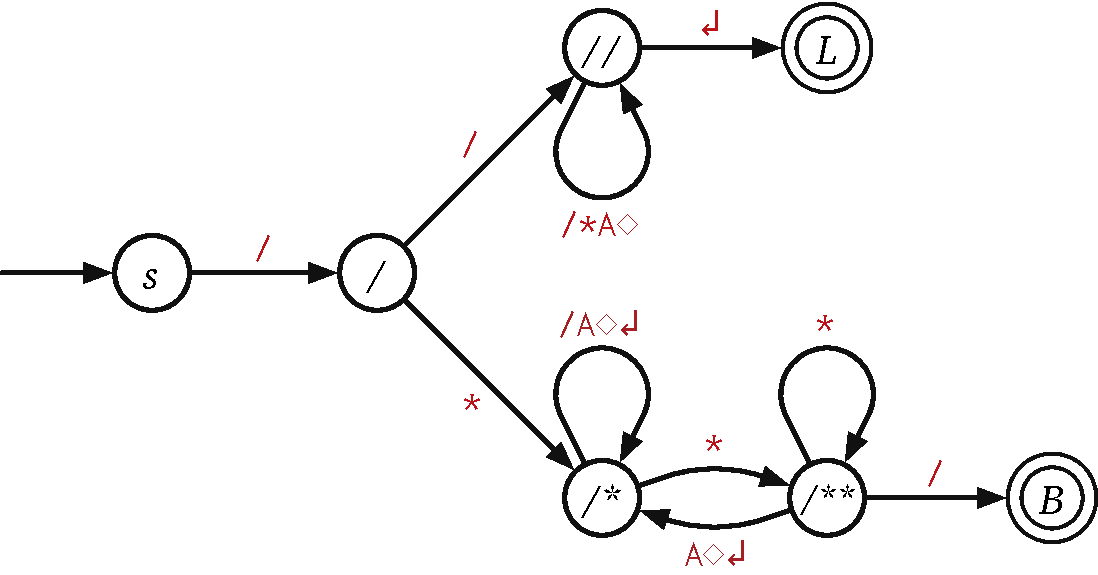
\includegraphics[scale=0.5]{../Fig/one-C-comment}
\end{center}
The states are labeled mnemonically as follows:
\begin{itemize}
\item $s$ — We have not read anything.
\item / — We just read the initial \Sym/.
\item // — We are reading a line comment.
\item $L$ — We have just read a complete line comment.
\item /* — We are reading a block comment, and we did not just read a \Sym* after the opening \Sym{/*}. 
\item /** — We are reading a block comment, and we just read a \Sym* after the opening \Sym{/*}. 
\item $B$ — We have just read a complete block comment. 
\end{itemize}
\end{Solution}
\unskip
\begin{rubric}
Standard DFA design rubric.  This is not the only correct solution, or even the simplest correct solution.  (We don’t need two distinct accepting states.)
\end{rubric}

\newpage
\item
Describe a DFA that accepts the set of all strings composed entirely of blanks (\Sym{\Blank}), newlines (\Sym{\Enter}), and C comments.

\begin{Solution}
By merging the accepting states of the previous DFA with the start state and adding white-space transitions at the start state, we obtain the following six-state DFA.  Again, all missing transitions lead to a hidden reject state.
\begin{center}
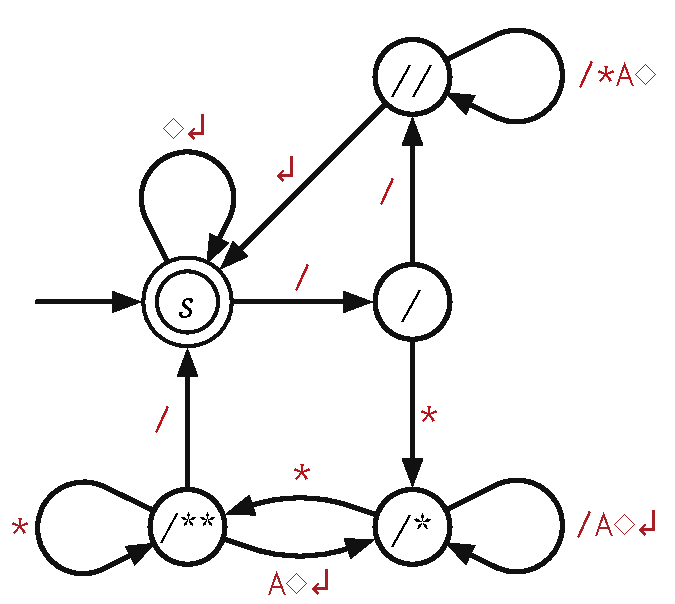
\includegraphics[scale=0.5]{../Fig/many-C-comments}
\end{center}
The states are labeled mnemonically as follows:
\begin{itemize}
\item $s$ — We are between comments.
\item / — We just read the initial \Sym/ of a comment.
\item // — We are reading a line comment.
\item /* — We are reading a block comment, and we did not just read a \Sym* after the opening \Sym{/*}. 
\item /** — We are reading a block comment, and we just read a \Sym* after the opening \Sym{/*}. 
\end{itemize}
\unskip
\end{Solution}
\unskip
\begin{rubric}
Standard DFA design rubric.  This is not the only correct solution, but it is the simplest correct solution.
\end{rubric}

\end{enumerate}

\end{enumerate}
 
%%%%%%%%%%%%%%%%%%%%
\end{document}

